\chapter{Resultados}

\section{Operacionalización de Variables}

En el presente trabajo se plantea la hipótesis: ...

\subsection{Variables Independientes}

Se tiene las siguientes ...

\subsection{Variables Dependientes}

De igual manera se tiene la ...

\section{Resultado experimentales}

\begin{figure}[H]
\caption{Comparación de mejores resultados para SURF entre la clasificación con y sin detección del danzante.}
\label{fig:chp-results:comp-results-SURF}
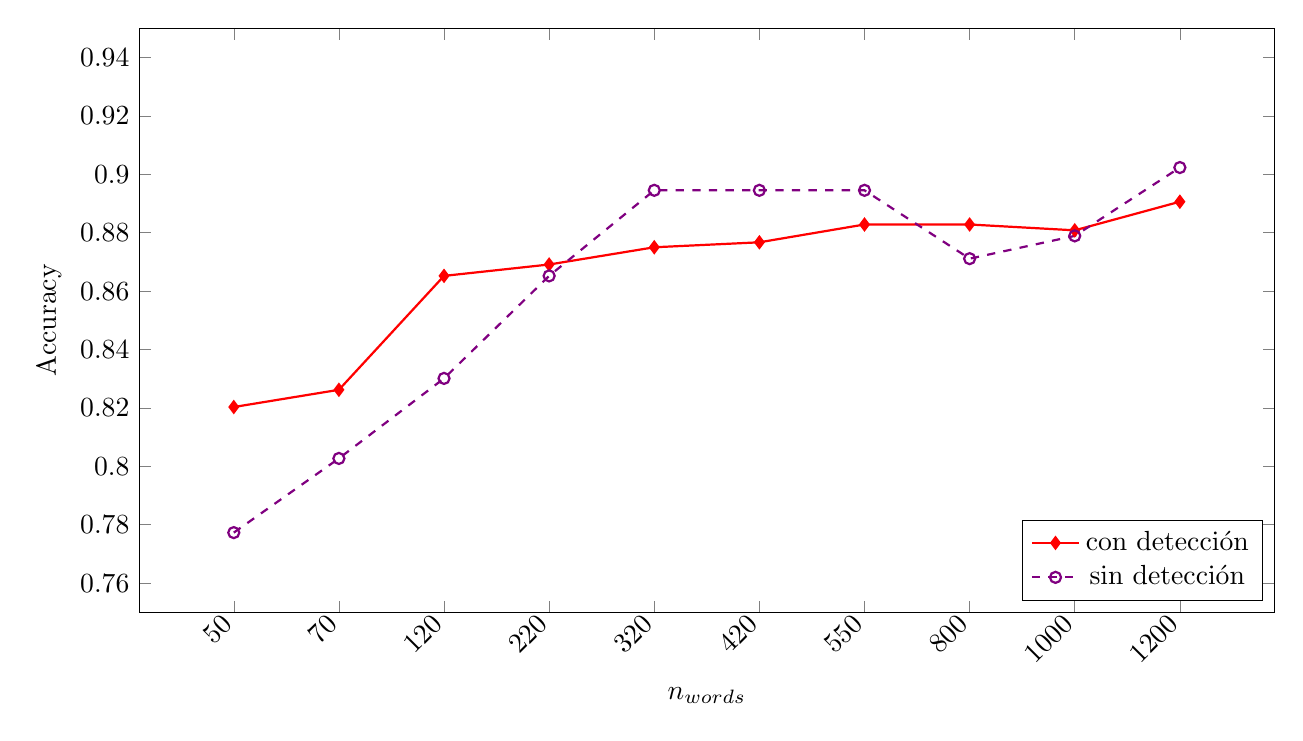
\begin{tikzpicture}
\begin{axis}[legend style={at={(0.99,0.02)},anchor=south east},
             symbolic x coords={50, 70, 120, 220, 320, 420, 550, 800, 1000, 1200}, xtick=data,
             x tick label style={rotate=45,anchor=east},
             ymin=0.75, ymax=.95,width=16cm,
            height=9cm, xlabel = $n_{words}$, ylabel = Accuracy
]

\addplot[mark=diamond*,thick,red] coordinates {
    (50, 0.8203)
    (70, 0.8262)
    (120, 0.8652)
    (220, 0.8691)
    (320, 0.8750)
    (420, 0.8767)
    (550, 0.8828)
    (800, 0.8828)
    (1000, 0.8808)
    (1200, 0.8906)
};
\addlegendentry{con detección}

\addplot[mark=o,mark options={solid},violet,thick,dashed] coordinates {
    (50, 0.7773)
    (70, 0.8027)
    (120, 0.8301)
    (220, 0.8652)
    (320, 0.8945)
    (420, 0.8945)
    (550, 0.8945)
    (800, 0.8711)
    (1000, 0.8789)
    (1200, 0.9023)
};
\addlegendentry{sin detección}

\end{axis}
\end{tikzpicture}
\end{figure}

\section{Contraste de Hipótesis}

Dado que en la operacionalización se define la variable \textbf{tasa de error de clasificación de imágenes de danzas típicas} en base a la ecuación ...

\section{Detalles Técnicos}
\label{detalles-tecnicos}

Para llevar a cabo el proyecto se hizo uso del siguiente hardware y software.

\subsection{Hardware}
\begin{itemize}
\item \textbf{Cámara:} Nikon D7200.
\item \textbf{Notebook:} Toshiba Satellite S845. Procesador Intel Core-i5 3rd generation/2.5 GHz, 4Gb RAM DDR3.
\item \textbf{Notebook:} Lenovo Y700. Procesador Intel Core-i7 6rd generation/3.5 GHz, 8Gb RAM DDR4.
\end{itemize}

\subsection{Software}
\begin{itemize}
\item \textbf{Sistema Operativo:} Ubuntu 16.04.1 LTS x86\_64 .
\item \textbf{Lenguaje de Programación:} Python 2.7 .
\item \textbf{Librerías:} Opencv 3.0.0, NumPy 1.11.2, SciPy 0.17.0, SciKitLearn 0.18 y SciKitImage 0.12.3.
\item \textbf{Controlador de versiones:} Git 2.10 .
\end{itemize}


